\documentclass[12pt]{article}

\setlength\parindent{0pt}
\newcommand{\myt}[1]{\textbf{\underline{#1}}}

\usepackage{mathtools}
\usepackage{amssymb}
\usepackage{graphicx}

\title{\vspace{-15ex}TITLE\vspace{-1ex}}
\date{May 4th, 2015}
\author{Graham Cooper}

\begin{document}
	\maketitle
	
	\section*{Dual Graphs}
	\myt{Definition:} Let G be a planar graph with an embedding. The dual G* of the embedding has one vertex $V_f$ corresponding to each face f of G, and foreach edge in G whose two sides are $f_1$, $f_2$, G* has a corresponding edge $V_{f_1}$, $V_{f_2}$.\\
	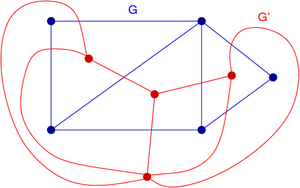
\includegraphics[scale=0.5]{dual.png}\\
	
	It is possible for the dual graph to have multiple edges and loops.\\
	
	\subsection*{Properties of Duality:}
	\begin{enumerate}
		\item IF G is planar then G* is also planar ( From inside a face, draw lines to the midpoints of the edges in the boundary)
		\item (G*)* = G
		\item \# of faces in G = \# of vertices in G*\\
				\# of vertices in G = \# of faces in G*\\
				\# of edges in G = \# of edges in G*
		\item degree of a vertex in G = deg of the corresponding face in G*\\
		degree of a face in G = degree of the corresponding vertex in G*
		\item The dual of a platonic graph is platonic
	\end{enumerate}
	
	\myt{Theorem:} The dual of an Eulerian planar graph is bipartite.\\
	
	\myt{Proof:} IF a graph is Eulerian, every vertex has even degree. So every face has even degree. By A9 last Question, the dual is bipartite.\\
	
	\section*{Matchings}
	\myt{Definition:} A matching of a graph is a  set of edges where no two edges share a common vertex (or they for ma subgraph of max dgeree 1)\\
	
	\myt{General Question:} What is the maximum size of a matching in a graph?\\
	
	\myt{Definition:} A vertex incident with an edge in a matching is called saturated. It is unsaturated otherwise.\\
	
	A matching that saturates all vertices is a perfect matching.\\
	
	If a graph has a perfect matching, then it has even \# of vertices.\\
	
\end{document}
